\documentclass[11pt]{article}

\usepackage{float}
\usepackage{hyperref}
\usepackage{graphicx}
% formatting
\usepackage{verbatim}
\usepackage{moreverb}
\usepackage{minted}
\usepackage{parskip}
\usepackage{amsmath}
\usepackage[listings]{tcolorbox}
\usepackage{enumerate}
\let\verbatiminput=\verbatimtabinput
\def\verbatimtabsize{4\relax}

\newcommand{\RepoRootPath}{fpga\_labs\_sp20}

\tcbset{
texexp/.style={colframe=black, colback=lightgray!15,
         coltitle=white,
         fonttitle=\small\sffamily\bfseries, fontupper=\small, fontlower=\small},
     example/.style 2 args={texexp,
title={Question \thetcbcounter: #1},label={#2}},
}

\newtcolorbox{texexp}[1]{texexp}
\newtcolorbox[auto counter]{texexptitled}[3][]{%
example={#2}{#3},#1}

\setlength{\topmargin}{-0.5in}
\setlength{\textheight}{9in}
\setlength{\oddsidemargin}{0in}
\setlength{\evensidemargin}{0in}
\setlength{\textwidth}{6.5in}

% Useful macros

\newcommand{\note}[1]{{\bf [ NOTE: #1 ]}}
\newcommand{\fixme}[1]{{\bf [ FIXME: #1 ]}}
\newcommand{\wunits}[2]{\mbox{#1\,#2}}
\newcommand{\um}{\mbox{$\mu$m}}
\newcommand{\xum}[1]{\wunits{#1}{\um}}
\newcommand{\by}[2]{\mbox{#1$\times$#2}}
\newcommand{\byby}[3]{\mbox{#1$\times$#2$\times$#3}}


\newenvironment{tightlist}
{\begin{itemize}
 \setlength{\parsep}{0pt}
 \setlength{\itemsep}{-2pt}}
{\end{itemize}}

\newenvironment{titledtightlist}[1]
{\noindent
 ~~\textbf{#1}
 \begin{itemize}
 \setlength{\parsep}{0pt}
 \setlength{\itemsep}{-2pt}}
{\end{itemize}}

% Change spacing before and after section headers

\makeatletter
\renewcommand{\section}
{\@startsection {section}{1}{0pt}
 {-2ex}
 {1ex}
 {\bfseries\Large}}
\makeatother

\makeatletter
\renewcommand{\subsection}
{\@startsection {subsection}{1}{0pt}
 {-1ex}
 {0.5ex}
 {\bfseries\normalsize}}
\makeatother

% Reduce likelihood of a single line at the top/bottom of page

\clubpenalty=2000
\widowpenalty=2000

% Other commands and parameters

\pagestyle{myheadings}
\setlength{\parindent}{0in}
\setlength{\parskip}{10pt}

% Commands for register format figures.

\newcommand{\instbit}[1]{\mbox{\scriptsize #1}}
\newcommand{\instbitrange}[2]{\instbit{#1} \hfill \instbit{#2}}
\newcommand{\itwos}{I\textsuperscript{2}S}

\begin{document}

\def\PYZsq{\textquotesingle}
\title{\vspace{-0.4in}\Large \bf EECS 151/251A FPGA Lab 5:\\FIFO with Ready/Valid Interfaces, HDMI Display\vspace{-0.1in}}

\author{Prof. John Wawrzynek \\
TAs: Quincy Huynh, Tan Nguyen \\ Department of Electrical Engineering and Computer Sciences\\
College of Engineering, University of California, Berkeley}
\date{}
\maketitle

\section{Before You Start This Lab}
You should run \verb|git pull| in \verb|fpga_labs_sp20| to get the latest files for this lab.

Before you proceed with the contents of this lab, we suggest that you get acquainted with what a \href{http://inst.eecs.berkeley.edu/~eecs151/sp20/files/verilog/ready_valid_interface.pdf}{ready/valid handshake} is. It may be helpful to draw out the timing diagrams for the ready/valid handshake to gain understanding. If you are having trouble, ask a TA. 

In this lab, we will build a FIFO with a Ready/Valid Interface, and we will learn how to use it for the task of streaming an image stored in FPGA memory to the HDMI output on the PYNQ board. \textbf{The FIFO module plays a significant role in the success of your final project, so you should make sure to test your FIFO implementation rigorously}. At least, it should be functionally working for some basic tests (we will see later). As this lab requires interfacing with a display device, you can use the lab monitors along with HDMI-to-VGA/HDMI-to-DVI adapters to test your designs. If you have a PYNQ board and a HDMI monitor home, you can also try it yourself. Please feel free to reach out to a TA if you are in need of any resources required to complete this lab.

\section{Building a Synchronous FIFO}
A FIFO (first in, first out) data buffer is a circuit that allows data elements to be queued through a write interface, and read out sequentially by a read interface.
The FIFO we will build in this section will have both the read and write interfaces clocked by the same clock; this circuit is known as a synchronous FIFO.

\subsection{FIFO Functionality}
A FIFO is implemented with a circular buffer (2D reg) and two pointers: a read pointer and a write pointer.
These pointers address the buffer inside the FIFO, and they indicate where the next read or write operation should be performed.
When the FIFO is reset, these pointers are set to the same value.

When a write to the FIFO is performed, the write pointer increments and the data provided to the FIFO is written to the buffer.
When a read from the FIFO is performed, the read pointer increments, and the data present at the read pointer's location is sent out of the FIFO.

A comparison between the values of the read and write pointers indicate whether the FIFO is full or empty.
You can choose to implement this logic as you please.
The \verb|Electronics| section of the \href{https://en.wikipedia.org/wiki/FIFO_(computing_and_electronics)}{FIFO Wikipedia article} will likely aid you in creating your FIFO.

For your reference, here is a block diagram of the Xilinx FIFO from page 103 of the \href{https://www.xilinx.com/support/documentation/ip_documentation/fifo_generator_ug175.pdf}{Xilinx FIFO IP Manual}.

\begin{center}
    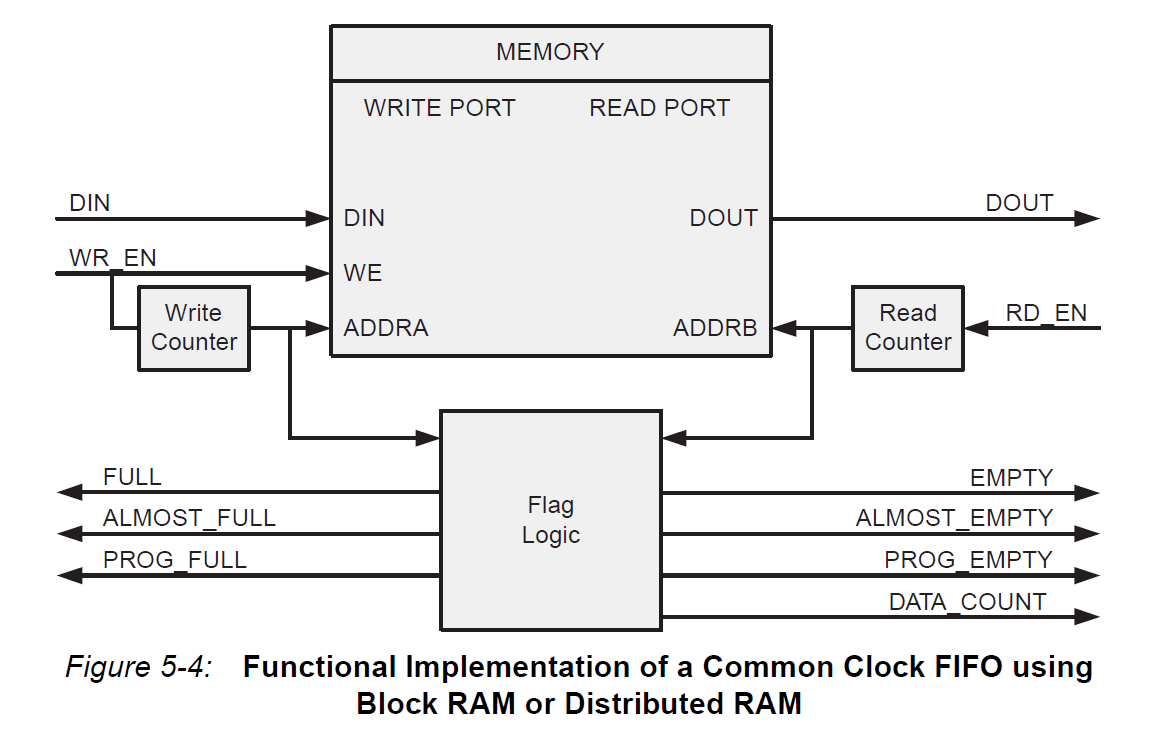
\includegraphics[height=7cm]{figs/sync_fifo_diagram.png}
\end{center}


Our FIFO, however, will have a much simpler interface than this. To make it convenient for you to connect your FIFOs with other Ready/Valid blocks in the future as well as to keep things consistent, our FIFO will also adopt the Ready/Valid Interface for the Read and Write channels. Since it might be read and written at the same time, we have to use a dual-ported memory block which supports two independent memory ports. We either use \verb|XILINX_SYNC_MEM_DP| or \verb|XILINX_ASYNC_MEM_DP| module from \verb|lib/EECS151.v| for our FIFO buffer. The difference between the two modules is the synchronous memory requires one-cycle read latency, whereas the read data of the asynchronous memory can be accessed immediately. You can take a look at their implementations for a better understanding. We use the synthesis attributes to enforce \verb|XILINX_SYNC_MEM_DP| to map to Block RAMs, while \verb|XILINX_ASYNC_MEM_DP| gets mapped to LUT RAMs on the FPGA, but the tool makes a final decision based on the availability of the resources. You can check with the Synthesis log file and the final report utilization to make sure you get what you want.


\begin{center}
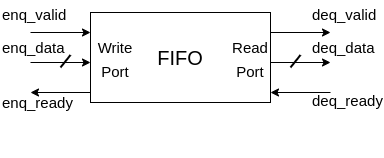
\includegraphics[width=0.6\textwidth]{figs/fifo.png}
\end{center}

\subsection{FIFO Interface}
Look at the FIFO skeleton in \verb|src/fifo.v|.

The FIFO is parameterized by:
\begin{itemize}
    \item \verb|WIDTH|    - The number of bits per entry in the FIFO
    \item \verb|LOGDEPTH| - The log2 of number of entries in the FIFO. For simplicity, our FIFO has a depth of power-of-two values.
\end{itemize}

The common FIFO signals are:
\begin{itemize}
    \item \verb|clk| - Clock used for both read and write interfaces of the FIFO.
    \item \verb|rst| - Reset (synchronous with \verb|clk|); should force the FIFO to become empty.
\end{itemize}

The FIFO write (or "enqueue") interface consists of:
\begin{itemize}
    \item \verb|input enq_valid| - If this signal is HIGH, the \verb|enq_data| is valid to be written to the FIFO (necessary, but not sufficient condition).
    \item \verb|input [WIDTH-1:0] enq_data| - the data to be written to the FIFO.
    \item \verb|output enq_ready| - If this signal is LOW, the FIFO is currently full. Nothing can be written to the FIFO. In other word, the FIFO is not ready to be enqueued/written to yet. \textbf{Use this signal to indicate whether the FIFO is full or not}.
\end{itemize}

The FIFO read (or "dequeue") interface consists of:
\begin{itemize}
    \item \verb|input deq_ready| - If this signal is HIGH, the \verb|deq_data| is ready to be read from the FIFO (necessary, but not sufficient condition).
    \item \verb|output [WIDTH-1:0] deq_data| - the data to be read from the FIFO.
    \item \verb|output deq_valid| - If this signal is LOW, the FIFO is currently empty. Nothing can be read from the FIFO. In other word, the \verb|deq_data| is an invalid data to be dequeued/read from the FIFO. \textbf{Use this signal to indicate whether the FIFO is empty or not}.
\end{itemize}

These signals work as similar to what you read from the \href{http://inst.eecs.berkeley.edu/~eecs151/sp20/files/verilog/ready_valid_interface.pdf}{ready/valid handshake} document. One way to imagine how it works is, for example, you can assume that the FIFO connects to a Source block (producing the data to the FIFO) on the Write interface, and a Sink block (consuming the data from the FIFO) on the Read interface. Therefore,

\begin{itemize}
    \item If \verb|enq_valid| and \verb|enq_ready| are both HIGH at a clock rising edge, the current data \verb|enq_data| from the Source block should be written/transferred to the FIFO at \textbf{the same} clock rising edge (enqueue "fired"). The write address increments at \textbf{the same} clock rising edge. Otherwise, nothing should be written to the FIFO.
    \item If \verb|deq_valid| and \verb|deq_ready| are both HIGH at a clock rising edge, the data \verb|deq_data| should be latched/transferred to the Sink block at \textbf{the same} clock rising edge (dequeue "fired"). The read address increments at \textbf{the same} clock rising edge. Otherwise, nothing should be read from the FIFO.
\end{itemize}

When you are confused whether a read or write transfer should happen, one tip is to always only look at the signal values right at a particular \textbf{rising edge}. Is Ready HIGH? Is Valid HIGH? If yes to both, the data on the FIFO data pin (\verb|enq_data| or \verb|deq_data|) is transferred at that rising edge. You don't really need to pay attention to how they change during that \textbf{clock cycle} prior to the rising edge. Read the linked document again to make sure you thoroughly understand how Ready/Valid interface works. If you're still in doubt, ask a TA for more clarification.

You can use either Asynchronous-Read memory (\verb|XILINX_ASYNC_MEM_DP|) or Synchronous-Read memory (\verb|XILINX_SYNC_MEM_DP|) as a buffer storage for your FIFO implementation. The latter might improve the maximum achievable frequency of your design, but it is more challenging to implement, since read is only updated at the next rising edge, i.e. the value that being written at this clock edge can only be available on the data output pin for read at the next clock edge. Due to such one-cycle delay, it is not possible to enqueue and dequeue the same data items in successive cycles if we only rely on the memory buffer; additional register might be needed to keep track of the current head of the FIFO.

You should try to implement a high-performance FIFO, i.e., there should be no cycle delay between any writes or reads in a row if the FIFO is not full or not empty, respectively.

\subsection{FIFO Testing}
We have provided a testbench in \verb|sim/fifo_testbench.v|.

The testbench performs the following test sequence:
\begin{enumerate}
    \item Checks initial conditions after reset (FIFO not full and is empty)
    \item Generates random data which will be used for testing
    \item Pushes the data into the FIFO, and checks at every step that the FIFO is no longer empty
    \item When the last piece of data has been pushed into the FIFO, it checks that the FIFO is not empty and is full
    \item Verifies that cycling the clock and trying to overflow the FIFO doesn't cause any corruption of data or corruption of the full and empty flags
    \item Reads the data from the FIFO, and checks at every step that the FIFO is no longer full
    \item When the last piece of data has been read from the FIFO, it checks that the FIFO is not full and is empty
    \item Verifies that cycling the clock and trying to underflow the FIFO doesn't cause any corruption of data or corruption of the full and empty flags
    \item Checks that the data read from the FIFO matches the data that was originally written to the FIFO
    \item Prints out test debug info
\end{enumerate}

Next are some harder tests:

\begin{itemize}
    \item Several times in a row, write to, then read from the FIFO with no clock cycle delays.
      This will test the FIFO in a way that it's likely to be used when buffering user I/O.

    \item Writing and Reading from the FIFO on the same cycle. We use fork-join to create parallel processes of writing and reading from the FIFO.
\end{itemize}

You should make sure that you pass all the tests before moving on.

\subsection{FIFO with IOs}

Your FIFO passes all the behavioral simulation tests. Well done! Next, we will make sure your FIFO is synthesizable by Vivado and it is actually working on an FPGA. We will do this by using the PYNQ IOs as both the source and the sink for the FIFO. In particular,

\begin{itemize}
    \item We use the buttons to enqueue data to the FIFO. Each \verb|BUTTONS[3:0]| corresponds to a number from 1 to 4.
    \item We use the LEDS to show the dequeued data.
    \item When SWITCHES[0] is OFF, it takes 0.5 second to dequeue an entry from the FIFO and display on the LEDS.
    \item When SWITCHES[0] is ON, the PYNQ is not ready to dequeue the data from the FIFO.
\end{itemize}

We have provided the code \verb|z1top_fifo_io.v| for you. Create a project with this file as top-level module and generate a bitstream to test it on the PYNQ. Make sure you add all necessary files (including the \verb|button_parser|, your FIFO code, and the constraint file). Alternatively, you can also run the script that we provide to interact with Vivado in command-line mode.

\begin{minted}{bash}
# This command creates 'z1top_fifo_io_proj' project, and then generates bitstream
# You should run the command under ./lab5 directory
make z1top_fifo_io

# This command loads the bitstream to a connected FPGA
make program-fpga bs=z1top_fifo_io.bit
\end{minted}

You can test your FIFOs by pressing different buttons, and keep track of the sequence of LEDS display to see if they match. Turn on SWITCHES[0] to try filling the FIFO until full, and then release SWITCHES[0] to drain the FIFO. You can as well modify the code to use SWITCHES[1] to prevent the FIFO from accepting new button input. In the next lab and project, your FIFO will receive user input from a keyboard and echo it back via a serial interface; anything can go wrong if your FIFO does not work reliably. It might be helpful to verify the functionality of your FIFO with this simple design beforehand, and you will have an easier time when working on the final project.


\section{HDMI Display}

In this section, we will ask you to build a display controller to interface with the HDMI output port on the PYNQ. Concretely, we stream a static image stored in the ROM of the FPGA to the display controller to the display monitor via HDMI interface. For this lab exercise, your display controller is expected to support a target resolution of 800$\times$600 with a frame-rate of 60Hz. This configuration should work with the monitors in the lab for check-off. As we move forward, you will find out that it is actually not difficult to build a parameterized display controller that can virtually support any resolution and frame-rate if we know all the necessary parameters and do the math right.

It might sound daunting at first, but we'd like to convince you that it is accomplishable thanks to the third-party \verb|rgb2dvi| IP from Digilent. The PYNQ HDMI ports (Input and Output) directly connect to the FPGA fabric via IO bank, and the \verb|rgb2dvi| IP is responsible for generating appropriate TMDS signals to the FPGA IOs that eventually interfaces with a HDMI sink monitor (or DVI). You can read more from the PYNQ documentation \href{https://reference.digilentinc.com/reference/programmable-logic/pynq-z1/reference-manual#hdmi}{HDMI}. You can also learn about the Digilent IP and how it is implemented from their Github repository. However, it is not required to know all the detail of the IP to actually use it. We just need to provide correct video-related signals to make the IP happy and do the work of streaming video data to the display device for us. Taking advantage of existing IPs saves countless hours of development effort. The signals that we pay attention to are:

\begin{itemize}
  \item \verb|vid_pData|: the three-color channel 24-bit video data. Each color channel has 8 bits. The color order is R, B, and G (from MSB to LSB).
  \item \verb|vid_pHSync|: the video Horizontal Syncing signal.
  \item \verb|vid_pVSync|: the video Vertical Syncing signal.
  \item \verb|vid_pVDE|: the video Enable signal (or video active).
\end{itemize}

Let's take a look at the following video timing figure (from \href{https://www.xilinx.com/support/documentation/ip_documentation/v_tc/v6_2/pg016_v_tc.pdf}{Xilinx Video Timing Controller document}) to understand where those signals come from.

\begin{center}
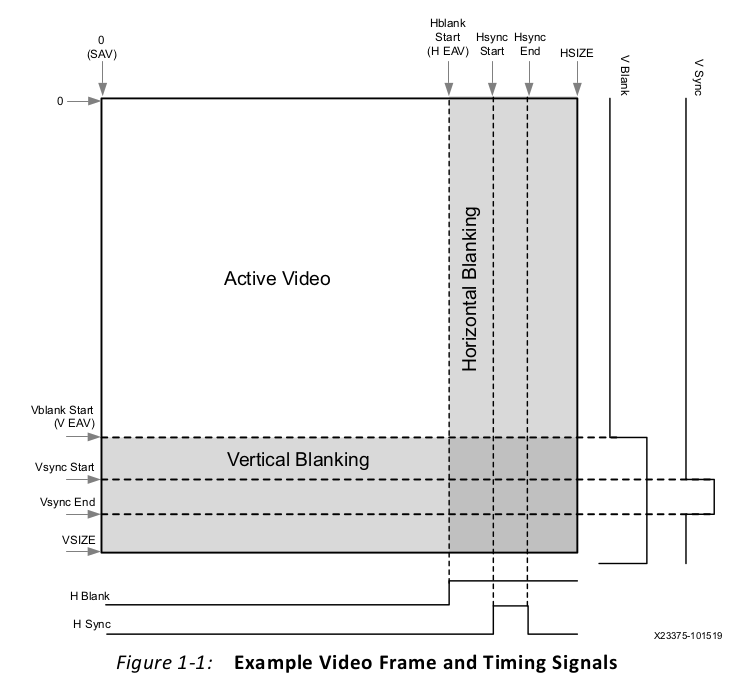
\includegraphics[width=0.8\textwidth]{figs/video_timings.png}
\end{center}

The figure defines the video timing parameters of a video frame. To understand it, you need to be aware that the way of how typical video display works is the pixels are rasterized/scanned from left-to-right, top-to-bottom. When the display scans a pixel within a region defined in the figure, we assert the corresponding signals accordingly. Note that the display resolution is actually the \verb|Active Video| region as seen in the figure. Therefore, there are some blanking periods in both horizontal and vertical direction that the display is not supposed to output thing. When you look at the spec of a particular display resolution, you will typically find the following parameters:

\begin{itemize}
  \item Horizotal Active Video: from 0 to the Width of the resolution, or HBlank Start.
  \item Horizontal Front Porch: from HBlank Start to HSync Start.
  \item Horizontal Sync Width: from HSync Start to HSync End.
  \item Horizontal Back Porch: from HSync End to HSIZE
  \item Vertical Active Video: from 0 to the Height of the resolution, or VBlank Start.
  \item Veritical Front Porch: from VBlank Start to VSync Start.
  \item Vertical Sync Width: from VSync Start to VSync End.
  \item Vertical Back Porch: from VSync End to VSIZE
\end{itemize}

Open the file \verb|lab5/src/display_controller.v|. You will see the parameters of different display configurations in the Verilog module parameter declarations. These parameters are the multiples of the \textbf{pixel clock cycle}. The pixel clock is calculated based on the target frame-rate/refresh-rate (e.g., a frame-rate of 60Hz means 60 frames per second) and the \textbf{entire video frame}. Note that a video frame includes both the active region and the blanking region. The pixel clock is the time it takes to emit a single pixel. Thus, with a total of frame\_rate $\times$ HSIZE $\times$ VSIZE pixels displayed in a second, a pixel clock can be calculated as 1 / frame\_rate $\times$ HSIZE $\times$ VSIZE second. As an example, for our target display resolution of 800$\times$600 @60Hz, the frame size is 1056x628 (including blanking regions), and the pixel clock is 25 ns or 40 MHz.

From these known parameters, we can calculate the syncing and blanking timings. As an example, HSync Start can be computed as Horizontal Active Video + Horizontal Front Porch, and Horizontal Sync End is HSync Start + Horizontal Sync Width.

To interface with the \verb|rgb2dvi| IP properly, we need to assert and deassert the \verb|HSync|, \verb|VSync|, and \verb|VDE| signals according to the spec. The \verb|HSync| should only be HIGH within the Horizontal Sync Width period (HSync Start $\rightarrow$ HSync End), the \verb|VSync| should only be HIGH within the Vertical Sync Width period (VSync Start $\rightarrow$ VSync End), and the \verb|VDE| should only be HIGH within the Active Video period (both horizontal and vertical). We don't care about VBlank or HBlank since the IP does not use these signals.

\subsection{Display controller with FIFO}

%\subsection{Display controller with test screen}


The following diagram depicts the system that we would like to run on the FPGA.

\begin{center}
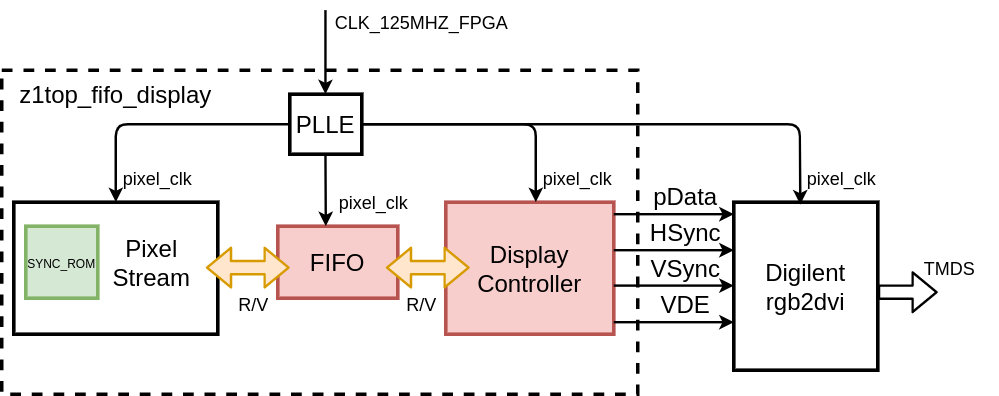
\includegraphics[width=0.6\textwidth]{figs/z1top_fifo_display.png}
\end{center}


The system consists of a pixel streaming block that sends pixel data of an image stored in a ROM every clock cycle to a FIFO. A display controller reads the pixel data from the FIFO and communicates with the Digilent IP to display image on a connected display device. You are responsible for the \verb|FIFO| and the \verb|display_controller| modules; the remaining blocks are provided to you and you should not need to modify them. Note that your \verb|FIFO| and \verb|display_controller| are now clocked with the pixel clock (40 MHz) instead of the system clock (125 MHz). The pixel clock is generated from the \verb|PLLE| module acting as a clock synthesizer to output a 40 MHz clock from an input 125 MHz clock. This module generates a more accurate frequency signals in comparison with the approach we took in the previous lab. We won't go into detail of it for now, but you should keep in mind that there are many ways to generate clock signals on the FPGA.

In summary, the \verb|pixel_stream| is a producer which sends a stream of pixels stored in the ROM to your FIFO. The \verb|display_controller| is a consumer which reads data from your FIFO if it is not empty, and generates video signals for the \verb|rgb2dvi| IP core. Since we are dealing with an IP, we won't be creating Vivado project by just adding Verilog files. Vivado also provides an \texttt{IP Integrator} feature allowing designers to connect their modules at a block level. We will discuss the process of doing IP integration in the Appendix section, for now, you can run the script that we provide you. It should create the projects with all the modules connected properly.

\begin{minted}{bash}
# This command creates 'z1top_fifo_display_proj' project, and then generates bitstream
# You should run the command under ./lab5 directory
make z1top_fifo_display
\end{minted}

You might want to open up the Vivado project to inspect what actually happens (or look at the script under \verb|lab5/scripts/z1top_fifo_display.tcl|. Click \emph{Open Block Design} under \emph{IP Integrator} to see the high-level overview of the design. If you successfully generate a bitstream, you can download it to an FPGA using the following command.

\begin{minted}{bash}
make program-fpga bs=z1top_fifo_display.bit
\end{minted}

Your \textbf{first task} is to implement a display controller in \verb|lab5/src/display_controller.v| that conforms to the video signal timings described above. You do not need to read from the FIFO for now, instead, you should write a constant video output (e.g., 24'h0000FF) to the \verb|rgb2dvi| module. \textbf{This should only require a few lines of code}. If you implement the video timing signals correctly, when you program the FPGA and hook it up with a monitor, it will display a blank green screen on the monitor (or a different color depending on which constant value). That means your display controller works properly. Good work! You can move on to the next part.

Next, your \textbf{second task} is to extend the display controller code to support a Ready/Valid interface that read pixel data from the FIFO. You are only required to modify the display controller, and you should use the FIFO code that you implement in the first section.

You don't need to worry about the implementations of other blocks in the system. That's the nice thing of Ready/Valid interface (often referred to as "Decoupled Interface" in other hardware construction language such as Chisel). All you need is to make sure your display controller can properly enqueue the incoming pixel data for video display, and stop the transfer during blanking periods. This test sytem also stresses your FIFO implementation in different ways as well, since there will be moments when the FIFO keeps writing and reading data continuously (during video active period), and there is some moment when the FIFO is buffering the data (during the video blanking periods). In addition, you don't need to worry about sizing your FIFO in the top-level module. In practice, even if your FIFO has a size of 1 or 2, this should still work since the \verb|pixel_stream| sends a pixel data every clock cycle. In a more complex system in which the producer's latency is unpredictable, you need to estimate the upper bound latency to size your FIFO accordingly, so that the pixel stream to the display is not halt which otherwise might cause unpleasant display experience. For now, we won't worry about this issue.

If you do everything right, you should see a static image on the monitor once you program the FPGA. Use the \verb|BUTTONS| to switch between different color channels. The image has a size of 800$\times$600. Since the block RAM resource on the FPGA is not adequate to hold 24-bit RGB 800$\times$600 image (which would require 800 $\times$ 600 $\times$ 24 / (18 $\times$ 1024) = 625 18Kb-BRAM blocks, way exceeds 280 18Kb-BRAM blocks available on our FPGAs). Hence, we convert the image to grayscale of 8-bit instead. Again, we hit the memory limit of our FPGA platform, this time for the display task, but let's leave this issue to another day, one thing for sure is your FIFO is good to go and you should be able to be checked off now.

\subsection{Real-time Graphics Drawing (Optional)}

You can try drawing interesting geomery objects to the display as well. Depending on how you implement the display controller, you might already be keeping track of the (x, y) pixel coordinates at each clock cycle, and you can decide how to color that pixel (the video output data) based on what you want to draw. Try drawing a few rectangles or triangles. You can use the buttons to change the coordinates to move the objects.

%\newpage
\section{Lab Deliverables (due: 11.59PM, Mar 5th, 2020)}
\subsection{Lab Checkoff}
To checkoff for this lab, have these things ready to show the TA:
\begin{enumerate}
  \item Demonstrate that your FIFO implementation passes all the simulation tests in the provided FIFO testbench.
  \item Demonstrate that your FIFO works properly with buttons, switches, and LEDs (\verb|z1top_fifo_io.v|).
  \item Demonstrate that your FIFO can receive the pixel stream and send the pixel stream to the display steadily ( \verb|z1top_fifo_display.v|).
\end{enumerate}

\subsection{Lab Report}\label{sec:labreport}

There is no report required for this lab.

\appendix
\section{Using Vivado IP Integrator}
Stay tuned.

\newpage
\section*{Ackowlegement}
This lab is the result of the work of many EECS151/251 GSIs over the years including:
\begin{itemize}
\item Sp12: James Parker, Daiwei Li, Shaoyi Cheng
\item Sp13: Shaoyi Cheng, Vincent Lee
\item Fa14: Simon Scott, Ian Juch
\item Fa15: James Martin
\item Fa16: Vighnesh Iyer
\item Fa17: George Alexandrov, Vighnesh Iyer, Nathan Narevsky
\item Sp18: Arya Reais-Parsi, Taehwan Kim
\item Fa18: Ali Moin, George Alexandrov, Andy Zhou
\item Sp19: Christopher Yarp, Arya Reais-Parsi
\item Fa19: Cem Yalcin, Rebekah Zhao, Ryan Kaveh, Vighnesh Iyer
\end{itemize}

\end{document}
